\documentclass{article}

% Packages
\usepackage{fullpage}
\usepackage{graphicx}
\usepackage{verbatim}

% Macros
% INSERT HW NUM HERE
\newcommand{\HWNUM}{2}

\begin{document}

    % TITLE SECTION

    \begin{center}
        ************************************ \\
        EE/CS 119A Homework \HWNUM \\
        Edward Speer \\
        \today \\
        ************************************
    \end{center}

    % PROBLEMS
    \begin{enumerate}
    
        \item \textbf{Problem 1}: \emph{Codebar Decoding} \\
        
            In order to simplify the logic of the codebar decoding, I began by
            developing a Python package which implements the Quine-McCluskey
            algorithm to find the prime implicants table of a given boolean
            function. I then wrote a script which used that package to find the
            prime implicant tables of each signal in the decoder. The code for
            that package and the script is attached at the back of the
            assignment. Use the chart to find the minimal sum of products
            representation of the function to cover all of the minterms, and
            reduce as much as possible.

            \begin{scriptsize}
                \begin{verbatim}
Signal: S
===============================
| I6...I0 |      Minterms    |
-------------------------------
| ...1.1. | x ||   || x || x |
-------------------------------
| .1.1... |   || x ||   ||   |
===============================
                \end{verbatim}
            \end{scriptsize}

            Trivially from the chart \fbox{$S=I_3 + I_1$}

            \begin{scriptsize}
                \begin{verbatim}
Signal: V3
========================================================
| I6...I0 |                Minterms                   |
--------------------------------------------------------
| ....1.1 |   ||   ||   ||   ||   || x ||   ||   || x |
--------------------------------------------------------
| ...1..1 | x ||   ||   ||   ||   ||   ||   ||   ||   |
--------------------------------------------------------
| ...11.. |   ||   ||   || x ||   ||   ||   ||   ||   |
--------------------------------------------------------
| ..1.... |   || x || x ||   || x ||   || x || x || x |
--------------------------------------------------------
| .0...01 | x ||   ||   ||   ||   || x || x ||   || x |
--------------------------------------------------------
| .0..10. |   ||   ||   || x ||   || x ||   || x || x |
--------------------------------------------------------
| .0.0.0. |   ||   ||   ||   ||   || x || x || x || x |
--------------------------------------------------------
| 0...0.0 |   || x || x ||   || x ||   ||   ||   ||   |
--------------------------------------------------------
| 0..1... | x ||   ||   || x || x ||   ||   ||   ||   |
--------------------------------------------------------
| 00...0. | x ||   ||   || x || x ||   ||   ||   || x |
--------------------------------------------------------
| 1.....1 |   ||   ||   ||   ||   || x || x ||   ||   |
--------------------------------------------------------
| 1...1.. |   ||   ||   ||   ||   || x ||   || x ||   |
========================================================
                \end{verbatim}
            \end{scriptsize}

            Here, one of the possible minimum covering sets may be made up of
            the one single term prime implicant plus the two double term prime
            implicants in rows 9 and 12. Thus \fbox{$V_3 = I_4 + I_6'I_3 + I_6I_2$}

            \pagebreak

            \begin{scriptsize}
                \begin{verbatim}
Signal: V2
========================================================
| I6...I0 |                Minterms                   |
--------------------------------------------------------
| ....1.1 |   ||   ||   ||   ||   || x ||   ||   || x |
--------------------------------------------------------
| ...1..0 |   ||   || x || x || x ||   ||   ||   ||   |
--------------------------------------------------------
| ...11.. |   ||   ||   || x ||   ||   ||   ||   ||   |
--------------------------------------------------------
| ..0.0.0 | x || x || x ||   ||   ||   ||   ||   ||   |
--------------------------------------------------------
| ..1...1 |   ||   ||   ||   ||   ||   || x ||   || x |
--------------------------------------------------------
| ..1.1.. |   ||   ||   ||   ||   ||   ||   || x || x |
--------------------------------------------------------
| ..11... |   ||   ||   ||   || x ||   ||   ||   ||   |
--------------------------------------------------------
| .0...00 |   ||   || x || x || x ||   ||   || x ||   |
--------------------------------------------------------
| .0..10. |   ||   ||   || x ||   || x ||   || x || x |
--------------------------------------------------------
| .0.0.0. |   ||   ||   ||   ||   || x || x || x || x |
--------------------------------------------------------
| .01..0. |   ||   ||   ||   || x ||   || x || x || x |
--------------------------------------------------------
| 1...... | x || x || x ||   ||   || x || x || x ||   |
========================================================
                \end{verbatim}
            \end{scriptsize}

            Here the minimum covering set may be made up of the one single term prime
            implicant plus the two double term prime impicants located in rows 1 and 2 of
            the table. Therefore \fbox{$V_2 = I_6 + I_3I_0' + I_2I_0$}

            \begin{scriptsize}
                \begin{verbatim}
Signal: V1
===============================
| I6...I0 |      Minterms    |
-------------------------------
| ....10. |   ||   || x ||   |
-------------------------------
| ...0.0. | x || x || x || x |
-------------------------------
| ..1..0. |   ||   ||   || x |
-------------------------------
| .1..... | x || x || x || x |
-------------------------------
| 0....00 |   ||   || x || x |
===============================
                \end{verbatim}
            \end{scriptsize}

            Trivially from the table \fbox{$V_1 = I_5$}

            \begin{scriptsize}
                \begin{verbatim}
Signal: V0
===============================
| I6...I0 |      Minterms    |
-------------------------------
| ......1 | x || x || x ||   |
-------------------------------
| ...1... |   || x ||   || x |
-------------------------------
| .0...0. |   || x ||   || x |
-------------------------------
| 0.0.0.. | x || x || x ||   |
===============================
                \end{verbatim}
            \end{scriptsize}

            Here the mimimal covering set may be formed by the two single term
            implicants in rows 1 and 2. Therefore \fbox{$V_0 = I_3 + I_0$}

            \pagebreak
            \begin{scriptsize}
                \begin{verbatim}
Signal: G
===============================================================================================================
| I6...I0 |                                                  Minterms                                        |
---------------------------------------------------------------------------------------------------------------
| 0.01001 |   ||   || x ||   ||   ||   ||   ||   ||   ||   ||   ||   ||   ||   ||   ||   ||   || x ||   ||   |
---------------------------------------------------------------------------------------------------------------
| 000.011 | x ||   ||   ||   ||   ||   ||   ||   ||   ||   ||   ||   ||   ||   ||   ||   ||   ||   || x ||   |
---------------------------------------------------------------------------------------------------------------
| 000.110 |   || x ||   ||   ||   ||   ||   ||   ||   ||   ||   ||   ||   ||   ||   ||   ||   ||   ||   || x |
---------------------------------------------------------------------------------------------------------------
| 00010.1 |   ||   || x ||   ||   ||   ||   ||   ||   ||   ||   ||   ||   ||   ||   ||   ||   ||   || x ||   |
---------------------------------------------------------------------------------------------------------------
| 00011.0 |   ||   ||   ||   ||   ||   ||   ||   ||   ||   || x ||   ||   ||   ||   ||   ||   ||   ||   || x |
---------------------------------------------------------------------------------------------------------------
| 001.010 |   ||   ||   ||   || x ||   ||   ||   ||   ||   ||   ||   ||   ||   ||   ||   || x ||   ||   ||   |
---------------------------------------------------------------------------------------------------------------
| 0010101 |   ||   ||   ||   ||   ||   ||   ||   ||   ||   ||   ||   ||   ||   ||   || x ||   ||   ||   ||   |
---------------------------------------------------------------------------------------------------------------
| 00110.0 |   ||   ||   ||   ||   ||   ||   ||   ||   ||   ||   || x ||   ||   ||   ||   || x ||   ||   ||   |
---------------------------------------------------------------------------------------------------------------
| 010.001 |   ||   ||   ||   ||   ||   || x ||   ||   ||   ||   ||   ||   ||   ||   ||   ||   || x ||   ||   |
---------------------------------------------------------------------------------------------------------------
| 0100100 |   ||   ||   ||   ||   ||   ||   || x ||   ||   ||   ||   ||   ||   ||   ||   ||   ||   ||   ||   |
---------------------------------------------------------------------------------------------------------------
| 0110000 |   ||   ||   ||   ||   ||   ||   ||   || x ||   ||   ||   ||   ||   ||   ||   ||   ||   ||   ||   |
---------------------------------------------------------------------------------------------------------------
| 1000010 |   ||   ||   ||   ||   || x ||   ||   ||   ||   ||   ||   ||   ||   ||   ||   ||   ||   ||   ||   |
---------------------------------------------------------------------------------------------------------------
| 1000101 |   ||   ||   ||   ||   ||   ||   ||   ||   ||   ||   ||   || x ||   ||   ||   ||   ||   ||   ||   |
---------------------------------------------------------------------------------------------------------------
| 1001000 |   ||   ||   ||   ||   ||   ||   ||   ||   || x ||   ||   ||   ||   ||   ||   ||   ||   ||   ||   |
---------------------------------------------------------------------------------------------------------------
| 1010001 |   ||   ||   ||   ||   ||   ||   ||   ||   ||   ||   ||   ||   || x ||   ||   ||   ||   ||   ||   |
---------------------------------------------------------------------------------------------------------------
| 1010100 |   ||   ||   ||   ||   ||   ||   ||   ||   ||   ||   ||   ||   ||   || x ||   ||   ||   ||   ||   |
---------------------------------------------------------------------------------------------------------------
| 1100000 |   ||   ||   || x ||   ||   ||   ||   ||   ||   ||   ||   ||   ||   ||   ||   ||   ||   ||   ||   |
===============================================================================================================
                \end{verbatim}
            \end{scriptsize}

            From the chart above, there is only one prime implicant which may be
            eliminated since almost all prime implicants are responsible for
            individual minterms. Row 1 may be eliminated. This results in:
            \[G = I_6'I_5'I_4'I_2'I_1I_0 + I_6'I_5'I_4'I_2I_1I_0' +
                  I_6'I_5'I_4'I_3I_2'I_0 + I_6'I_5'I_4'I_3I_2I_0' +
                  I_6'I_5'I_4I_2'I_1I_0' + I_6'I_5'I_4I_3'I_2I_1'I_0\]\[ +
                  I_6'I_5'I_4I_3I_2'I_0' + I_6'I_5I_4'I_2'I_1'I_0 +
                  I_6'I_5I_4'I_3'I_2I_1'I_0' + I_6'I_5I_4I_3'I_2'I_1'I_0' +
                  I_6I_5'I_4'I_3'I_2'I_1I_0' + I_6I_5'I_4'I_3'I_2I_1'I_0 + \]\[
                  I_6I_5'I_4'I_3I_2'I_1'I_0' + I_6I_5'I_4I_3'I_2'I_1'I_0 +
                  I_6I_5'I_4I_3'I_2I_1'I_0' + I_6I_5I_4'I_3'I_2'I_1'I_0\]

            Combining terms and simplifying slightly:
            \[G = I_6'I_5'I_4'(I_2 \oplus I_0)(I_1+I_3) + I_6'I_5'I_4(
                  I_2'I_1I_0' + I_3'I_2I_1'I_0 + I_3I_2'I_0') +
                  I_6'I_5I_4'(I_2'I_1'I_0 + I_3'I_2I_1'I_0') + \]\[
                  I_6'I_5I_4I_3'I_2'I_1'I_0' + I_6I_5'I_4'(I_3'I_2'I_1I_0' + 
                  I_3I_2'I_1'I_0' + I_3'I_2I_1'I_0) + I_6I_5'I_4I_3'I_1'(I_2
                  \oplus I_0) + \]\[I_6I_5I_4'I_3'I_2'I_1'I_0'\]

            The logic for each of these signals is implemented in 61.5 gates in
            the following circuit, which was checked using a python script also
            attached at the back of the assignment.

            Note that for the circuit drawn, in order to reduce gate count using
            negative logic, the inverters on each of the inputs have both matched
            and unmatched bubbles. Since they were being used across multiple
            inputs, it was not possible to match bubbles correctly without using
            additional inverters. Therefore I placed all of the bubbles on the 
            input inverters in a consistent manner, and then ensured the bubble
            rules were followed throughout the rest of the design.

            \begin{center}
                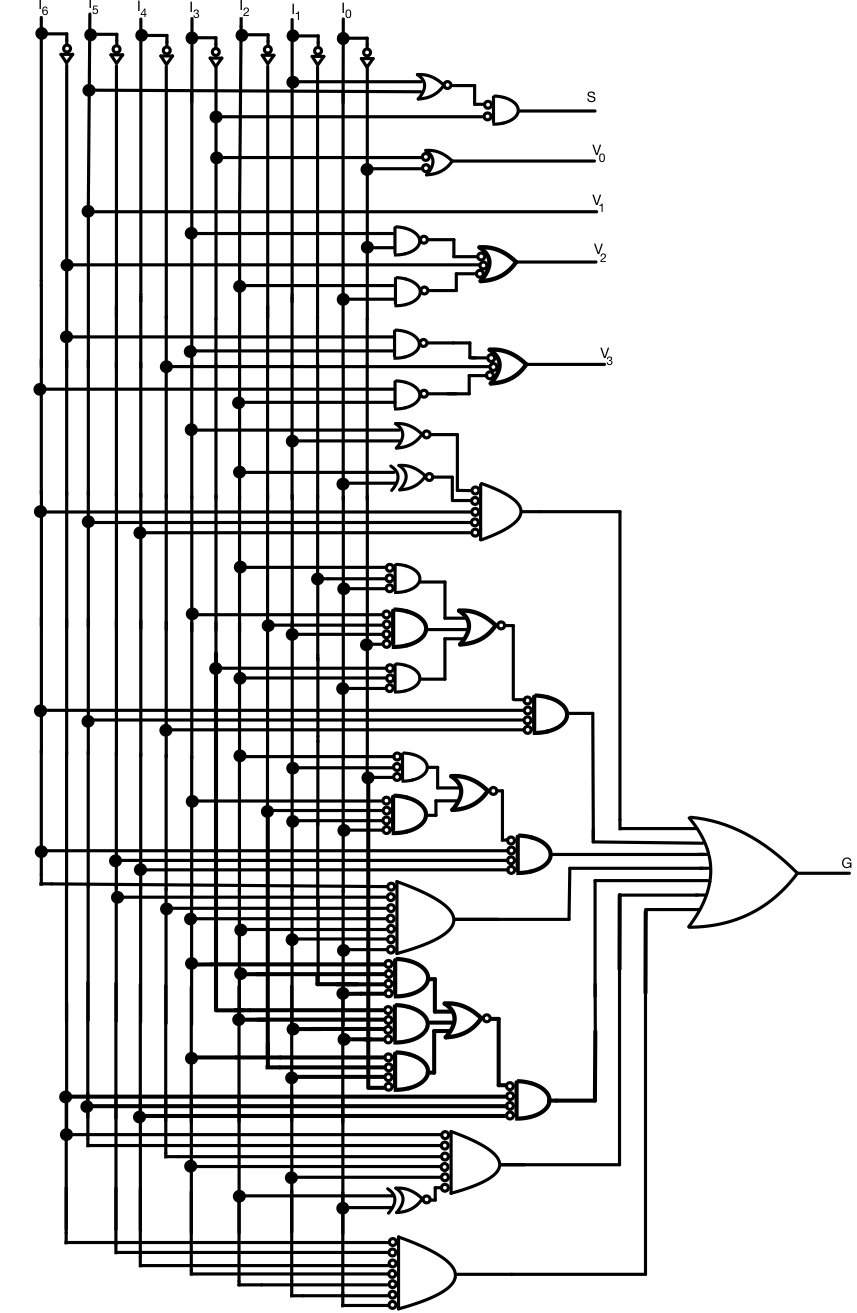
\includegraphics[width=0.85\textwidth]{figs/p1.jpeg}
            \end{center}

        \item \textbf{Problem 2}: \emph{Glitches} \\
            
            In order to have a potential glitch in the circuit, we need a case
            where the transition of a signal impacts the output of multiple
            gates concurrently. In this circuit, we have 3 gates, meaning we
            have 3 pairings of gates to consider.

            \begin{itemize}
                \item Consider the first and second product terms. The first
                contains $C$ while the second contains $C'$. This means there
                is a potential for a glitch on the transition of $C$ if we can 
                produce an input for which the output of the whole circuit
                relies on the value of $C$ in gates 1 and 2. Consider the input 
                1110. In this case, the second product term will start out high,
                while the first and third are low. When $C$ transitions to low, 
                the output should remain high. However, the output of the second 
                gate will transition to low before the output of the first gate
                goes high due to the propagation delay of $C$ through the
                inverter, meaning that the output of the circuit would
                temporarily glitch low even though it should stay high.
                \item Consider the first and third product terms. The first term
                holds $B$ while the third holds $B'$. This means there is a
                potential for a glitch on the transition of $B$ if we can
                produce an input for which the output of the whole circuit
                relies on the value of $B$ in gates 1 and 3. Consider the input
                1101. In this case, the first product term will start out high,
                while the second and third are low. When $B$ transitions to low,
                the output should remain high. However, the output of the first
                gate will transition to low before the output of the third gate
                goes high due to the propagation delay of $B$ through the
                inverter, meaning that the output of the circuit would
                temporarily glitch low even though it should stay high.
                \item Consider the second and third product terms. The second 
                term is actually the NOT of the third term, meaning that no one 
                input could cause a swap of the outputs of these gates. This
                means that there is no potential for a glitch between these two 
                gates with a single signal transition.

            \end{itemize}

        Therefore, the potential values for which the circuit may glitch when a
        signal transitions are 
        
        \fbox{(1110 $\leftrightarrow$ 1100) and (1101
        $\leftrightarrow$ 1001)}

        To resolve these glitches, we can collect the common terms in the glitch
        conditions into a redundant term for each glitch condition, therefore
        placing an extra gate which will reamin high on the transition and
        thus mask the glitch by holding the output high. 

        \begin{itemize}
            \item For the transitions $1110 \leftrightarrow 1100$, this means we
                  should add the product term $AB\overline{D}$ which will remain
                  high regardless of the transition of $C$.
            \item For the transitions $1101 \leftrightarrow 1001$, this means we
                  should add the product term $A\overline{C}D$ which will remain
                  high regardless of the transition of $B$.
        \end{itemize}

        This gives us a final circuit with 5 product terms, described by the
        following equation:
        
        \fbox{$Y = (A*B*\overline{C}) + (B*C*\overline{D}) +
               (\overline{B}*\overline{C}*D) + (A*B*\overline{D}) +
               (A*\overline{C}*D)$}

        \pagebreak

    \item \textbf{Problem 3}: \emph{Gate counts} \\
    
        Count the number of gates in the circuit part by part.

        \begin{itemize}
            \item U29 is a 74LS00, a quad 2-input NAND gate, giving 4 gates.
            \item U19, U20, and U21 are 74LS04s, hex inverters, giving
                  $6+0.5 = 3$ gates, times 3 is 9 gates.
            \item U33 is a 74AHCT1G04, a single half-gate inverter.
            \item U9-U15 and U32 are 74LS08, quad 2-input AND gates, giving
                  $4 * 1.5 = 6$ gates, time 8 is 48 gates.
            \item U25-U28 are 74LS11, triple 3-input AND gates, giving
                  $2 * 3 = 6$ gates, times 4 is 24 gates.
            \item U31 is a 74LS20, a dual 4-input NAND gate, giving 4 gates.
            \item U22-U24 are 74LS27, triple 3-input NOR gates, giving
                  $1.5 * 3 = 4.5$ gates, times 3 is 13.5 gates.
            \item U16-U18 are 74LS32, quad 2-input OR gates, giving
                  $1.5 * 4 = 6$ gates, times 3 is 18 gates.
            \item U6 is a 74LS83, given in handout as 31 gates.
            \item U30 is a 74LS85, given in handout as 22.5 gates.
            \item U1 and U5 are 74LS92, given in handout as 21 and 27 gates
                  respectively.
            \item U7 and U8 are 74LS175, quad D flip-flops with clear. These
                  yield 4 DFFs * 6 gates per DFF, plus an additional gate for
                  an inverter and a buffer each, giving 25 gates per package,
                  times 2 is 50 gates.
            \item Now, subtract away the unused gates, a two input AND from U14,
                  a two input AND from U32, and a two input OR from U18. This is
                  -4.5 gates.
        \end{itemize}

        In total, this is $4 + 9 + 0.5 + 48 + 24 + 4 + 13.5 + 18 + 31 + 22.5 + 
        21 + 27 + 50 - 4.5 = $ \fbox{268 gates}

    \end{enumerate}

    \pagebreak
    \verbatiminput{../Q-M/qm.py}
    \pagebreak
    \verbatiminput{p1.py}
    \pagebreak
    \verbatiminput{check_1.py}

\end{document}
